\documentclass{article}
\usepackage{graphicx, hyperref}
\usepackage{float}
\bibliographystyle{elsarticle-num}

\graphicspath{ {images/} }

\newcommand{\projectnaam}{Software Reengineering}
\newcommand{\student}{Van Muylder Ben \& Geeraert Lander}
\title{\textmd{\textbf{Final Project Report}}\\\normalsize\vspace{0.1in}\Large{\projectnaam}}
\author{\student}\date{\today}

\setcounter{section}{-1}

\begin{document}
\maketitle
\newpage

\section{Introduction}

\subsection{Context}

This project is part of the course 'Software Reengineering' at the University of Antwerp. It serves (to quote the assignment) "to demonstrate that you indeed acquired the range of principles, techniques, and skills that are currently being used for reengineering", and such we will need to (and we'll again quote the assignment) "restructure an existing software system to prepare for a given suite of new requirements".

\subsection{Do reengineer, do not implement}

As you can read in the above part, we are required to prepare the software system 'for a given suite of new requirements', hence we are not required to implement these features, as is confirmed by yet another excerpt from the assignment: 'the extra functionality as such needs not be implemented; but [...] the existing design must be adjusted in such a way that adding the new functionality becomes a [...] piece of cake".\\

We want emphasize that we will \textbf{not} be implementing the features as they were noted in the assignment (those being: having the functionality to have separate shapes for data points, and having the functionality to read shapes for data point from a database).

\subsection{Problem at hand} 

The problem which we should try to grasp is the following: a hypothetical customer wants us to refactor the existing software library 'JFreeChart'. To be more precise, he wants us to refactor the library as to allow for functionality which the library currently does not have. This functionality (as mentioned before) is a) to allow for separate shapes for data points and b) to allow for the loading of shapes from a database.

\section{Preparation}

\subsection{Scope}

The assignment is directed at a very specific part of the library. While there is no functionality to explicitly give each separate datapoint a specific shape, there is already functionality for datapoints to have shapes (which was to be expected). While there are very much aspects to this library, many of which could perhaps require their own refactoring, we will only focus on the functionality concerning shapes. Throughout the report we might refer back to this limit as our scope.

\section{Design Recovery}

To understand what should be changed in the project, we must first understand how the project works. Since our scope is the functionality of shapes, we must thus try to work out what the role of these shapes is, and how precisely they work.

\subsection{Analysis of the current design}

We'll be honest and upfront in saying that we won't have a whole explanation of how this library works, but rather a simplified view of happens in general, concerning to our scope (with possible deeper insights in those aspects which need more explanation).\\

A shape can be used for many things, but with respect to the assignment; it's used to represent a datapoint on a plot. A datapoint can be a point of its own, or it can be part of a set of datapoints (which we mostly refer to as a serie). This serie might represent a lot of things such as just simply random points, points of data which have been imported, points which represent a (mathematical) function... 

However, purely in data, a shape does not have not much meaning. The shape itself is meant so we, the user of the library, can see these points on a screen. And when does this happen? When we export our plot (and data) to an image (for example).\\

This is where our overview of the workings begin. When we want to export to an image, we'll want to output some data to a buffer. The output comes from a draw function which is a central part of the core functionality, which in itself calls the draw functionality of the Plot interface (which is implemented by XYPlot and CategoryPlot among others...). These draw funtions do a lot of things, but one thing in particular: they render data items, or at least, set this process into motion. XYPlot for example has its own render function, which then in itself calls to the drawItem function of the renderer for that class instance (which would be an XYItemRenderer, which is in itself an interface, but is implemented in a lot of derived classes such as XYLineAndShapeRenderer). The drawItem functionality of XYLineAndShapeRender works with different passes: a first pass which draws the background, and a second pass which draws effective data items.\\

We have now reached the point where we will effectively have interaction with shapes. For simplicity we'll say that the draw function of these classes effectively \textit{draws} the shapes somewhere. But to do this, the function needs a shape to draw. They do this by calling the getItemShape function of AbstractXYItemRenderer or AbstractCategoryItemRenderer (which both inherit this function from AbstractRenderer, and which both are extended by lots of other classes, such as XYLineAndShapeRenderer). This function provides and effective shape which the draw function then can use to \textit{draw}.

getItemShape is special in 2 ways. The first way is in that it will always return the same shape for data items of the same serie (because of the deeper implementation of this function). The second way is that it is called in many other classes (which are thus extensions of AbstractXYItemRenderer and AbstractCategoryItemRenderer); unlike the function setSeriesShape (and setItemShape, which is a function which doesn't exist (yet)).\\

The function to set a specific shape for a serie (also part of AbstractRenderer), is never used in the whole project. But plots still need shapes for their data points? This is where default shapes come in play. Classes can set a shape by either changing the value for the default shape in the constructor, or by setting a shape for the series legend and then later on requesting the shape of the data point via the shape of the legend of that serie. 

\section{Design}

\subsection{The initial idea}

When figuring out how the current implementation of the library works, we noticed one thing in particular. While the library does not have the functionality which is requested by our metaphorical customer, it still possible without the need for grand refactors and restructurings of the project.\\

For example: in the above part we spoke specifically of the function getItemShape, and not of the function getSeriesShape. This is because getItemShape is meant to return a specific shape for each separate datapoint, while getSeriesShape is meant to return a shape for each separate serie. In practice, the second parameter of getItemShape (which would denote the specific point of a serie for which we want to get a shape) is completely ignored, after which getSeriesShape is called.\\

getItemShape in this case serves purely as a passthrough function, where it is explicitly mentioned in the documentation for the function that if other behaviour is required, the users should override the existing function. This however, doesn't seem to happen anywhere in the project and thus we can safely say that getItemShape effectively is the same as lookupSerieShape (which in itself calls getSeriesShape).\\

Because of this, in our opinion, the project does not need refactoring to allow for the requested features, not even to make the implementation easier, as implementing it would only require the getItemShape function to be overridden correctly. One could even write an implementation for getItemShape where they perform a specific database query (based on the row and column parameter of getItemShape) to request a specific shape from a database.\\

Nevertheless, we'll try and find more opportunities to restructure the project to allow for more ease of use.

\subsubsection{Pulling away the shape functionality}

While we think that the shape functionality itself does not need changing to allow for the requested features, we do think that it is not easy for people who are not familiar with the project to effectively find where the functionality of the shapes resides (which is in the AbstractRenderer class).\\

Because of this we propose to pull away this functionality from the AbstractRenderer class, and put it inside of it's own class (which we will call ShapeManager) and make AbstractRenderer extend from it, simply to provide more clarity and to make the functionality easier to find. As such, the following are diagrams of how the current implementation of AbstractXYItemRenderer is and how the current implementation of AbstractCategoryItemRenderer is.

\begin{figure}[H]
\centering
	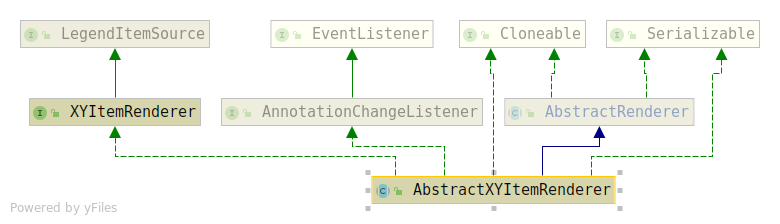
\includegraphics[width=0.9\textwidth]{AbstractXYItemRendererBefore.png}
	\caption{AbstractXYItemRenderer before any refactorings}
\end{figure}

\begin{figure}[H]
\centering
	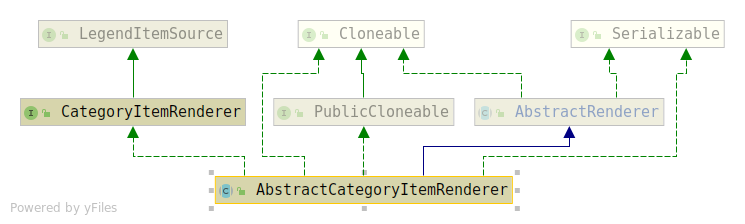
\includegraphics[width=0.9\textwidth]{AbstractCategoryItemRendererBefore.png}
	\caption{AbstractCategoryItemRenderer before any refactorings}
\end{figure}

What is important to note from these figures, is that AbstractRenderer (the class where the shape functionality resides) has not further dependencies. This is what will change in our proposed design.
As such, the following are diagrams of how our proposed implementation is for AbstractXYItemRenderer and AbstractCategoryRenderer.

\begin{figure}[H]
\centering
	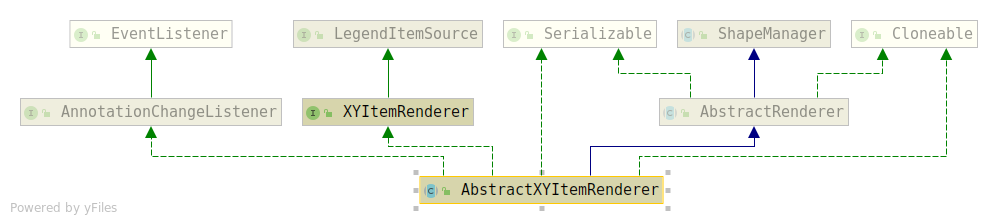
\includegraphics[width=0.9\textwidth]{AbstractXYItemRendererAfter.png}
	\caption{AbstractXYItemRenderer after refactoring}
\end{figure}

\begin{figure}[H]
\centering
	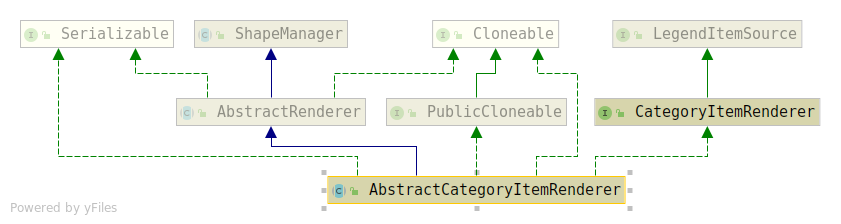
\includegraphics[width=0.9\textwidth]{AbstractCategoryItemRendererAfter.png}
	\caption{AbstractCategoryItemRenderer after refactoring}
\end{figure}

To reiterate; we want to perform this refactor purely for the sake of clarity, to help our (hypothetical) customer with figuring out where he should start with the implementation of his new functionality.

\subsubsection{Risks}

Since we simply want to pull away the functionality, and put it in a class from which the original class will extend, we effectively make sure that our original class doesn't change (since a compiled version will use flattened versions for classes, having the original class extend from the class with the functionality, makes it so that our original class (which is AbstractRenderer) keeps the functionality which we pulled away).\\

As such it fairly clear that there aren't much risks involved with performing this refactor. Nevertheless, we should at least a) check with an IDE whether we have created errors and b) rerun the existing test suite. If the test suite fails, there is a problem. However, if it succeeds this can mean either that everything still works, or that the existing test suite is not capable and produced a false positive. Nevertheless, we'll assume that we started with a stable version of the library, which has a capable test suite.


\subsection{Other possibilities}

Now that we know that we don't need to refactor the project \textbf{to allow for the requested funtionality}, we can go looking at what can be optimized in the general sense of refactoring. But this raises another problem. Since we localized the current functionality (and the place where the future functionality would or could be placed) of the project to being a very precise spot, the effective code scope of this assignment has been greatly reduced. Either we try to refactor the functionality which we plan to extract from AbstractRenderer, or we expand our scope.\\

After some hefty discussing, we agreed that expanding our scope, would make the scope drift too far from the assignment. Thus, we'll initially extract the shape functionality from the AbstractRenderer, after which we look how this extracted functionality can be further refactored.


\section{Management}

Due to the nature of our workflow, you might already have guessed that there is not much planning and managing to do on with our current plan. The greater part of what we did was mostly discussing whether what we were doing was the right thing to do.\\

In other cases using a Ghantt or Pert chart might be a useful tool, but in our case the work which has to be done should only take a mere minutes, since it's mostly cut and paste work. Nevertheless this doesn't mean that we shouldn't have to check the changes that we made.

\section{Restructuring}

\subsection{Refactoring}

\subsubsection{Results - Duplicate Code}

We used 2 tools to look for code duplication, Intelij and Iclones. Both had confusing results.\\

First we ran the tools on a version of Jfreechart without the refactor to have a baseline to compare to. We saw that Iclones found a lot of duplicates. These can be found in the clonereportbefore.txt file. We expect that this will only increase because we literally copied some functions. Thus effectively introduced a new duplicate.\\

After running Iclones on the recent version of JfreeChart (one where the refactor was done) we saw a surprising result. The amount of duplicates found had drastically been reduced. Which we found odd because of the aforementioned duplicate we introduced.\\

To try clarify these results we ran also duplicate detection with Intelij. This gave similar results but was easier to navigate and analyze. Here we discovered that some duplicates didn't show up because of a low complexity or severity.\\

We theorize that thanks to the refactor. A lot of duplicates get less severe or complex. That in turn makes them not show up in the results of duplicate analysis. Another clarification could be that the heuristic used during duplicate analysis somehow doesn't recognize the same duplicates anymore.\\
\subsubsection{Results - Coverage}

We ran coverage reports before and after we performed our shape functionality extraction (moved them to our ShapeManager class), which gave us some surprising results. While we didn't expect much of the coverage to change (since in theory almost everything stays the same) except for some minor details concerning the classes/packages which were directly linked to AbstractRenderer, but the results show us some strange changes.\\

For example; some other packages seem to have gained some classes (chart.axis) while other packages seem to have lost some classes (data.json, data.json.impl, chart.text).

\newpage
\begin{figure}[H]
\centering
	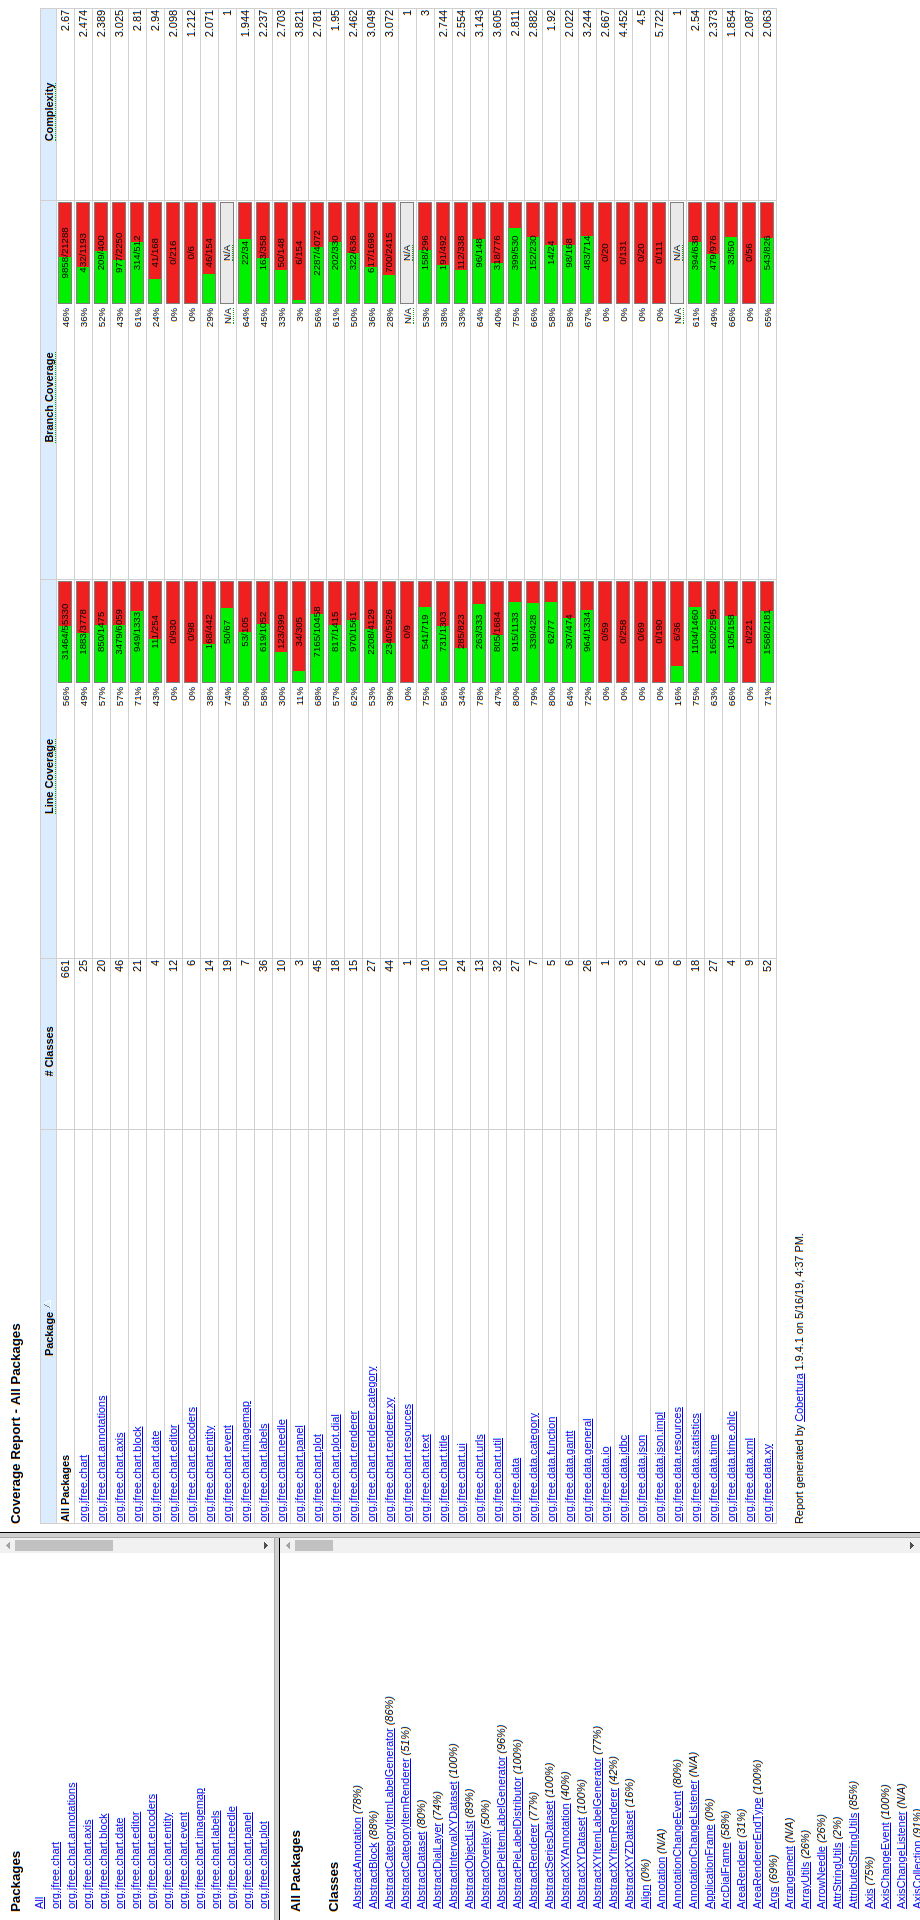
\includegraphics[width=0.7\textwidth]{coverage/BEFORE.png}
	\caption{coverage before extraction}
\end{figure}

\newpage
\begin{figure}[H]
\centering
	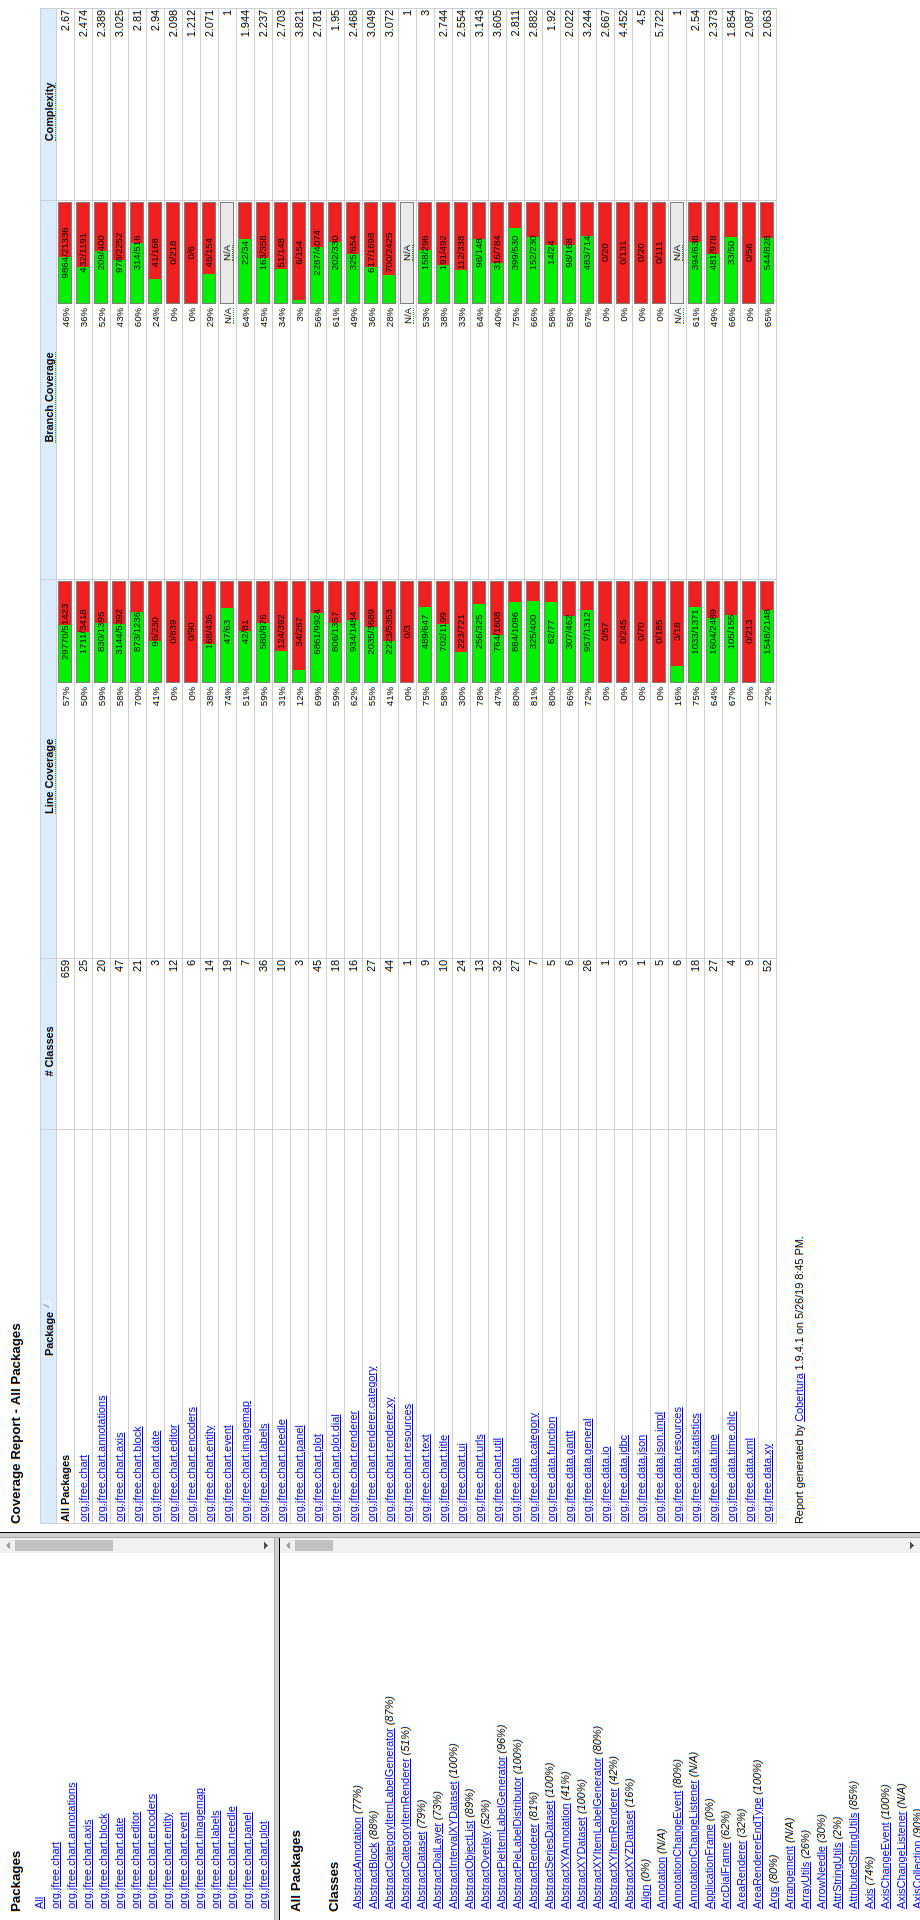
\includegraphics[width=0.7\textwidth]{coverage/AFTER.png}
	\caption{coverage after extraction}
\end{figure}

\subsection{Testing}


\newpage
\section{Conclusion}

We want to begin our conclusion with a well known saying: "If it aint broke, don't fix it." The problem with this quote is that it is often used as an excuse for not touching a working piece of software, which may still be broken in some way.\cite{mps}\\ 

The second thing we want to mention in our conclusion is yet again our scope. Simply said, we had to refactor the project as to allow the requested functionality to be implemented. So the first (big) question we asked ourselves was: what should be refactored to allow for this functionality to be implemented? When we finally figured out how the system worked, our first remark was: \textit{this project doesn't need to be refactored to allow for the requested functionality}.\\

But this doesn't mean that everything in the system is optimal. So since our first step was to 'refactor the system as to allow for the requested behavior', the second step would be 'check whether the system (within our working scope) has other optimization we can realize'. So after evaluating whether our scope had to be expanded (which we eventually didn't), we began perfoming some analysis techniques on this extracted functionality.

\subsection{Remarks}

For us, this project consisted mostly of discussing what might be the right thing to do in this case. We came to a fairly quick conclusion that we thought the project should not be refactored to allow for the requested behaviour. Of course, this seemed a bit strange to us, so there was a lot of discussing whether or not that was the right thing to do. We opted to make the functionality concerning shapes more visible to anyone who would actually want to implement the requested functionality. But this was a mere cut and paste job for us. So once again we discussed whether this was enough, was this all we could do to try and achieve our goal.\\

We tried to stand in the shoes of the 'customer'. Whether he would be satisfied if we presented him our final result. It was a tricky situation, because from the customers point of view, he wants to receive the library in a state where it is possible for him (or someone else) to actually implement those features, but we would be there to tell him: "It is already possible. It might not be that clear that it is already possible, so made it a bit clearer." So eventually we decided that our hypothetical customer would indeed be satisfied.\\

There has been a lot of discussing, about a lot of things, some of them being: what is our scope, when are we not doing enough, when are we going out of scope... But one thing in particular: What is the line between refactoring (preparing the project to allow for the implementation of the requested features) and implementing (actually readying the code for this implementation). We agreed that it was not our place to decide how a third person would or should implement those features, which led to being our biggest holdback in  doing things during this project. Yes, we could have made a database interface to \textit{portray that reading shapes from a database would be fairly easy}, or we could have effectively implemented some version of the getItemShape (and setItemShape), but other than serving as unfinished examples just to prove our point it would be useless. If our explanation cannot prove our point, than we probably are just explaining it wrong.

\subsection{Notes}

\subsubsection{Tool Usage}

In this section we'll list all the tools which we used to become our results for this assignment.

\begin{itemize}
	\item Jetbrains IntelliJ\newline usage: code editing, code inspection, feature location, duplicate detection, code smells, refactoring
	\item CodeScene\newline usage: code smells, refactoring targets, general project analysis
	\item iClones\newline usage: duplicate detection
	\item SonarCloud\newline usage: bug detection, duplicate detection, code smells, general analysis
	\item Cobertura (included with the project)\newline usage: coverage analysis
\end{itemize}

\newpage
\bibliography{mybibfile}


\end{document}